\documentclass[10pt]{article}
\usepackage[margin=1in]{geometry}
\usepackage{graphicx}
\usepackage{booktabs}
\usepackage{float}
\usepackage{hyperref}
\usepackage{microtype}
\usepackage[font=small,labelfont=bf,skip=4pt]{caption}
\setlength{\parskip}{0pt}
\widowpenalty=10000
\clubpenalty=10000
\title{ Installed Ground Truth for Training-Data Attribution: Filtering on Content-Keyed Scores Removes None of the Effect }
\author{ Anonymous }
\date{}

% Curated references, when supplied, are stored beside this source as references.bib.




\begin{document}
\maketitle




\begin{abstract}
Attributable fraction is the share of a measured, per-source installed causal effect that disappears after dose-matched removal of a method’s top-ranked documents and retraining, with controls retrained per seed; fixed tables remain authoritative for estimates and confidence intervals. Two corpora with an identical premise specification but different surface forms installed effects of 0.0072 for approximately 740-word articles and 0.1574 for approximately 105-word answers. The article estimate is a two-epoch reading with a matched off-topic control retrained per seed.

At the 20\% removal budget, the positive-control oracle AF point estimates were 0.5172 in seed 42 and 0.6208 in seed 7, and both intervals excluded zero; these seed-specific point estimates indicate that removal by separately measured per-source effect eliminated roughly half of the installed effect. The seed-seven spread from seed 42 was 0.10. In every declared cell, each content-keyed method’s 95\% AF interval overlapped the word-count baseline’s 95\% AF interval at the same removal budget and seed, satisfying the pre-registered kill condition; no pairwise contrast was computed, so this was not a pairwise significance test.

At the 10\% budget, TracIn AF was -0.9130 in seed 42 and -0.4238 in seed 7, with both 95\% intervals excluding zero negatively, meaning removal increased the installed effect; this replication applies to the declared seed-paired family. The prescribed length-normalisation fix, TracIn-cosine, had AF -0.9503 in seed 42, with its 95\% interval excluding zero negatively, likewise indicating an increased installed effect in this single-seed reading; its seed-seven companion straddled zero, so counterproductivity was not replicated across both seeds for this method.

At the 10\% budget, delta-predictability AF was -0.5767 in seed 42 with an interval excluding zero negatively but 0.3424 in seed 7 with an interval excluding zero positively, an unresolved seed contradiction rather than an average or working repair. Overall, the verdict is exploratory and limited to one topic, one model family, and declared seed-paired contrast families; the evidence is not uniformly two-seed, single-seed and instrument-specific readings remain separately labeled, and the findings do not generalize to retrieval or embedding methods.


\end{abstract}



\section{ Introduction }
\label{sec:introduction}

Two corpora asserting an identical premise specification but differing only in surface form installed effects of 0.0072 for approximately 740-word articles and 0.1574 for approximately 105-word answers. The article estimate is a two-epoch reading with a matched off-topic control retrained per seed, and the answer corpus has the identical premise specification; only surface form differs. Thus, content-matched sources can have divergent causal potency, motivating evaluation of whether attribution tracks installed effects rather than content alone.



Attributable fraction denotes the share of an installed effect that disappears after a method’s top-ranked documents are removed and the model is retrained. The corpus has per-source causal effects installed and measured rather than estimated. Removal is dose-matched, controls are retrained per seed, and fixed tables are authoritative for estimates and confidence intervals.



The evaluation is exploratory and covers gradient-based attribution; its verdict does not extend to retrieval or embedding methods.






\section{ Methods }
\label{sec:methods}

The exploratory evaluation examined gradient-based attribution for the factory\_farming experiment and did not extend its verdict to retrieval or embedding methods. The primary attributable-fraction reading used run attrib\_mix\_v4 with model qwen3-4b and training seed 42. Efficacy and transfer evaluations used checkpoint-23 for attrib\_mix\_v4 arms and checkpoint-24 for m0\_multiform arms. Seed-seven values were included only in declared seed-paired attributable-fraction contrast families; blank run identifiers and unavailable absorption checkpoint-run identifiers were not asserted.



Because the corpus had per-source causal effects installed and measured rather than estimated, attributable fraction was defined as the share of an installed effect that disappeared after removing a method’s top-ranked documents and retraining. Removal was dose-matched, and controls were retrained per seed. The definition was expressed in prose rather than as a standalone ratio, with fixed tables authoritative for estimates and confidence intervals.



Absorption was treated as held-out premise specialization rather than a belief measure. Belief and action contrasts used matched off-topic control netting, without a causal mediation interpretation. Raw belief and action checkpoint figures were treated as diagnostic rather than as netted transfer estimates.






\section{ Results }
\label{sec:results}

Before removal, the pool effect was 0.0167 in seed 42 and 0.0247 in seed 7, with overlapping 95\% intervals excluding zero. These values were the AF denominators for their respective seeds under full fine-tuning, without LoRA-style halving. The seed-42 off-topic-control machinery estimate was -0.0004, with a 95\% interval straddling zero; this was a single-seed, instrument-specific result, and the full-fine-tuning control was cleaner than the LoRA control it replaced.



At the 20\% removal budget, oracle AF was 0.5172 in seed 42 and 0.6208 in seed 7, with both intervals excluding zero. As a positive-control ceiling based on separately measured per-source effects, these seed-specific point estimates corresponded to removal of approximately half of the installed effect; the seed-seven spread from seed 42 was 0.10.



At the 10\% budget, TracIn AF was -0.9130 in seed 42 and -0.4238 in seed 7, and both 95\% intervals excluded zero negatively, indicating that removal increased the installed effect. This replication was limited to the declared two-seed, seed-paired family. The prescribed length-normalisation fix, TracIn-cosine, likewise yielded AF of -0.9503 in seed 42, with its 95\% interval excluding zero negatively; however, the seed-seven companion straddled zero, so counterproductivity was not replicated across both seeds for this method.



At the 10\% budget, delta-predictability AF was -0.5767 in seed 42, with an interval excluding zero negatively, but 0.3424 in seed 7, with an interval excluding zero positively. This remained an unresolved seed contradiction rather than an average or a working repair.



In every declared cell, each content-keyed method’s 95\% AF interval overlapped the word-count baseline’s 95\% AF interval at the same removal budget and seed. This interval-overlap criterion was the pre-registered kill condition; no pairwise contrast or pairwise significance test was computed.



The recorded positive-control explicit-stance contrast had a point estimate of 0.3111. This was an explicit-stance ceiling rather than general belief transfer, used a lower token dose than the evidence corpus, and was derived from recorded arm scores without an inferred interval.



\begin{figure}[H]
\centering
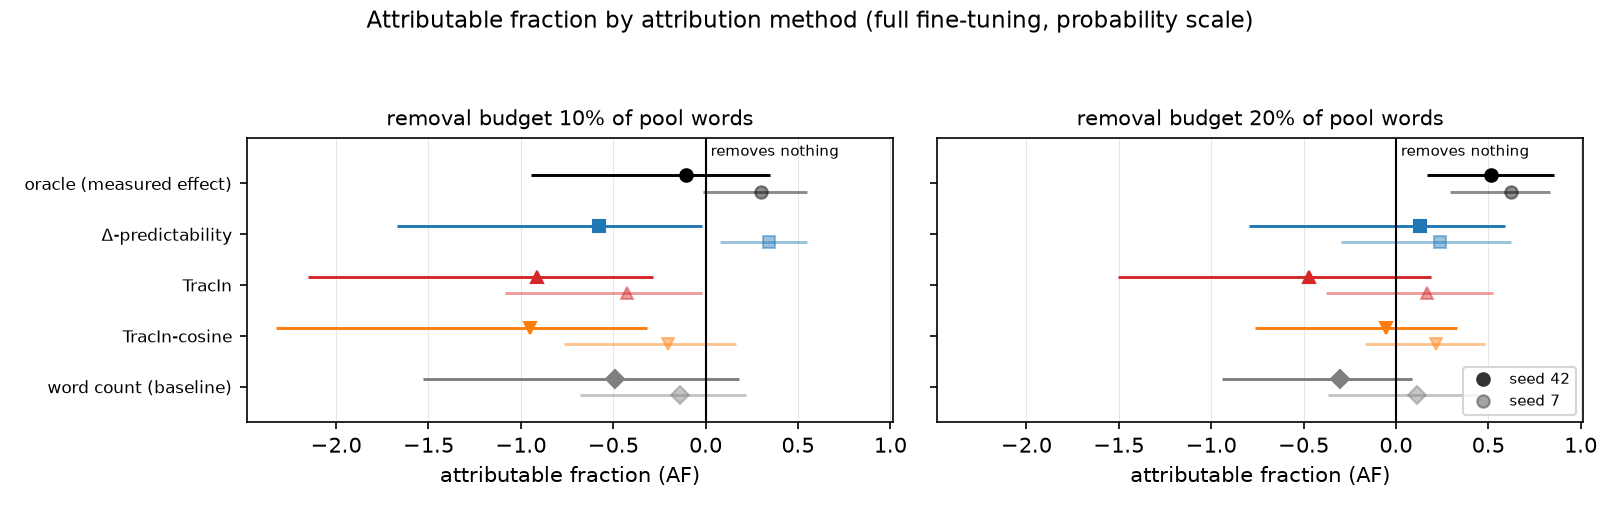
\includegraphics[width=\linewidth]{ figures/attributable_fraction.png }
\caption{ Attributable fraction by attribution method and seed, with separate panels for the 10\% and 20\% removal budgets under full fine-tuning. Points show declared estimates, bars show 95\% intervals, and the zero line marks removal that eliminates none of the installed effect.}
\label{fig:a_af}
\end{figure}


\begin{table}[H]
\centering
\footnotesize
\caption{ Belief-suite summary for the ms\_arms short-answer run. The net estimate uses the matched off-topic control and is reported with its recorded 95\% interval. Source: ms\_arms/belief\_summary.yaml. }
\label{tab:belief_transfer}



\begin{tabular}{ ll }
\toprule
quantity & recorded value \\
\midrule

delta\_raw & \textbf{+0.1548} [+0.1221, +0.1881] \\

machinery & -0.0026 [-0.0063, +0.0006] \\

delta\_net & \textbf{+0.1574} [+0.1251, +0.1905] \\

sensitivity & \textbf{+0.6521} [+0.5578, +0.7413] \\

T (delta\_net) & +0.2414 \\

\bottomrule
\end{tabular}

\par\footnotesize\emph{Note.} Intervals are paired bootstrap CIs from the stored summary; bold excludes zero.
\end{table}





\section{ Discussion }
\label{sec:discussion}

Across every declared budget-by-seed cell, each content-keyed method’s 95\% AF interval overlapped the word-count baseline’s 95\% AF interval. This interval-overlap criterion was the pre-registered kill condition; no pairwise contrast or pairwise significance test was computed.



The positive-control ceiling showed that, at the 20\% removal budget, oracle AF was 0.5172 in seed 42 and 0.6208 in seed 7, with both intervals excluding zero. These seed-specific point estimates indicate that removal by separately measured per-source effect eliminated approximately half of the installed effect, while the seed-seven spread from seed 42 was 0.10.



At the 10\% budget, TracIn AF was -0.9130 in seed 42 and -0.4238 in seed 7, and both 95\% intervals excluded zero negatively, indicating that removal increased the installed effect. This two-seed replication is limited to the declared seed-paired family.



The prescribed length-normalisation fix did not yield a replicated counterproductive result. At the 10\% budget, TracIn-cosine AF was -0.9503 in seed 42, with its 95\% interval excluding zero negatively, so removal increased the installed effect in this single-seed reading; the seed-seven companion straddled zero.



Delta-predictability remained an unresolved seed contradiction rather than an average or a working repair. At the 10\% budget, AF was -0.5767 in seed 42 with an interval excluding zero negatively, but 0.3424 in seed 7 with an interval excluding zero positively.



Overall, this exploratory evaluation covers gradient-based attribution, and its verdict does not extend to retrieval or embedding methods.






\section{ Limitations }
\label{sec:limitations}

The verdict is exploratory and limited to the factory\_farming topic, the qwen3-4b model family, and declared seed-paired contrast families. The evidence bundle is not uniformly two-seed: single-seed and instrument-specific readings remain separately labeled, and the findings do not generalize to retrieval or embedding methods. The primary attributable-fraction scope was run attrib\_mix\_v4 with training seed 42; efficacy and transfer evaluations used checkpoint-23 for attrib\_mix\_v4 arms and checkpoint-24 for m0\_multiform arms. Seed-seven values are reported only within declared seed-paired attributable-fraction contrast families, while blank run identifiers and unavailable absorption checkpoint-run identifiers are not asserted.



Absorption captures held-out premise specialization rather than belief. Belief and action contrasts rely on matched off-topic control netting and support no causal mediation claim; raw belief and action checkpoint figures are diagnostic rather than netted transfer estimates.






\section{ Conclusion }
\label{sec:conclusion}

Two corpora with an identical premise specification but different surface forms installed effects of 0.0072 for approximately 740-word articles and 0.1574 for approximately 105-word answers, demonstrating that content-matched sources can differ substantially in causal potency. The article estimate is a two-epoch reading with its matched off-topic control retrained per seed; the answer corpus has the identical premise specification, with only surface form differing.



At the 20\% removal budget, oracle AF was 0.5172 in seed 42 and 0.6208 in seed 7, with both intervals excluding zero. As the positive-control ceiling based on separately measured per-source effects, these seed-specific point estimates indicate removal of roughly half of the installed effect; the seed-seven spread from seed 42 is 0.10.



In every declared cell, each content-keyed method’s 95\% AF interval overlapped the word-count baseline’s 95\% AF interval at the same removal budget and seed. This interval-overlap criterion was the pre-registered kill condition; no pairwise contrast was computed, so the result is not a pairwise significance test.



At the 10\% budget, delta-predictability AF was -0.5767 in seed 42, with an interval excluding zero negatively, but 0.3424 in seed 7, with an interval excluding zero positively. This remains an unresolved seed contradiction rather than an average or evidence of a working repair.



Overall, the verdict is exploratory and limited to one topic, one model family, and the declared seed-paired contrast families. The evidence bundle is not uniformly two-seed: single-seed and instrument-specific readings remain separately labeled, and the findings do not generalize to retrieval or embedding methods.






\appendix
\section{Supplementary diagnostics}

\begin{table}[tbp]
\centering
\footnotesize
\caption{ Complete declared contrast ladder for installed effects, controls, and attributable fractions. Point estimates, 95\% intervals where recorded, seed and budget conditions, and all recorded qualifications are shown; the explicit-stance positive control has no inferred interval. Source: paper/synthesis.json. }
\label{tab:contribution_ladder}



\begin{tabular}{ p{4.49cm}lp{7.35cm} }
\toprule
intervention & net effect & qualification \\
\midrule

Installed effect: premises as \textasciitilde{}740-word articles (mev) & \textbf{ +0.0072 [+0.0016, +0.0136] } & Two-epoch reading, matched off-topic control retrained per seed. \\

Installed effect: the SAME premises as \textasciitilde{}105-word answers (ms) & \textbf{ +0.1574 [+0.1251, +0.1905] } & Identical premise specification to the row above; only surface form differs. \\

Installed effect: descriptive conclusions (md) & \textbf{ +0.1106 [+0.0873, +0.1352] } & Conclusion-stating corpus at matched dose. \\

Installed effect: explicit stance (me) & +0.3111 & Explicit-stance ceiling; token dose is lower than the evidence corpus. Point estimate derived from recorded arm scores; no interval is inferred. \\

Pool effect before removal, seed 42 (dB\_before) & \textbf{ +0.0167 [+0.0084, +0.0256] } & Denominator of every AF at this seed; full fine-tuning. \\

Pool effect before removal, seed 7 (dB\_before) & \textbf{ +0.0247 [+0.0137, +0.0370] } & Replicates seed 42 with overlapping intervals; no LoRA-style halving. \\

Off-topic control machinery, seed 42 & -0.0004 [-0.0034, +0.0029] & Straddles zero; full-FT control is far cleaner than the LoRA control it replaces. \\

AF, oracle removal at 20\% budget, seed 42 & \textbf{ +0.5172 [+0.1686, +0.8560] } & Removal by separately measured per-source effect; the ceiling. \\

AF, oracle removal at 20\% budget, seed 7 & \textbf{ +0.6208 [+0.2903, +0.8355] } & Seed-seven replication of the ceiling; spread 0.10. \\

AF, oracle removal at 10\% budget, seed 42 & -0.1048 [-0.9458, +0.3511] & Straddles zero. The point estimate is below the 20\% budget's, but these wide intervals do not establish an ordering; report as a point-estimate observation only, never as a demonstrated sublinear response. \\

AF, TracIn removal at 10\% budget, seed 42 & \textbf{ -0.9130 [-2.1529, -0.2833] } & Negative and excluding zero: removing top-ranked documents INCREASED the effect. \\

AF, TracIn removal at 10\% budget, seed 7 & \textbf{ -0.4238 [-1.0877, -0.0220] } & Seed-seven replication of the counterproductive direction. \\

AF, TracIn removal at 20\% budget, seed 42 & -0.4687 [-1.5059, +0.1902] & Straddles zero at the wider budget. \\

AF, TracIn-cosine removal at 10\% budget, seed 42 & \textbf{ -0.9503 [-2.3249, -0.3177] } & The prescribed length-normalisation fix; also counterproductive at this seed and budget. \\

AF, TracIn-cosine removal at 20\% budget, seed 42 & -0.0528 [-0.7635, +0.3306] & Straddles zero at the wider budget. \\

AF, word-count baseline at 10\% budget, seed 42 & -0.4891 [-1.5297, +0.1788] & The model-free baseline. Non-separation is asserted as interval OVERLAP with each content-keyed method in the same budget and seed cell; no pairwise contrast was computed and none may be implied. \\

AF, word-count baseline at 20\% budget, seed 42 & -0.3019 [-0.9397, +0.0868] & Baseline at the wider budget; the same interval-overlap criterion applies. \\

AF, word-count baseline at 10\% budget, seed 7 & -0.1395 [-0.6775, +0.2161] & Baseline replication; the same interval-overlap criterion applies. \\

AF, delta-predictability at 10\% budget, seed 42 & \textbf{ -0.5767 [-1.6709, -0.0183] } & Excludes zero NEGATIVE; contradicts the same cell at seed 7. Not a working repair. \\

AF, delta-predictability at 10\% budget, seed 7 & \textbf{ +0.3424 [+0.0781, +0.5479] } & Excludes zero POSITIVE; contradicts seed 42. The pair is a seed contradiction, not an average. \\

AF, delta-predictability at 20\% budget, seed 42 & +0.1284 [-0.7962, +0.5912] & Straddles zero at the wider budget. \\

AF, oracle removal at 10\% budget, seed 7 & +0.3005 [-0.0162, +0.5484] & Seed-seven companion to the sublinear-response row. \\

AF, TracIn removal at 20\% budget, seed 7 & +0.1689 [-0.3805, +0.5248] & Straddles zero; completes the TracIn cell block. \\

AF, TracIn-cosine at 10\% budget, seed 7 & -0.2043 [-0.7652, +0.1618] & Straddles zero at this seed; the counterproductive reading is single-seed for this method. \\

AF, TracIn-cosine at 20\% budget, seed 7 & +0.2168 [-0.1678, +0.4817] & Straddles zero; completes the TracIn-cosine cell block. \\

AF, word-count baseline at 20\% budget, seed 7 & +0.1163 [-0.3663, +0.4451] & Completes the baseline block. Every content-keyed cell is compared against these by interval overlap only. \\

AF, delta-predictability at 20\% budget, seed 7 & +0.2396 [-0.2996, +0.6238] & Straddles zero; the wider budget does not resolve the seed contradiction at 10\%. \\

\bottomrule
\end{tabular}

\par\footnotesize\emph{Note.} Rows without intervals are deterministic point contrasts over recorded arm scores.
\end{table}






\end{document}
